\chapter{Dedução da equação \ref{eq:positivity_prop}}
\label{append:proof-positive-p}

Neste apêndice, provamos a existência da distribuição de momentos magnéticos positiva $p(x'', y'', z_{c})$ que resolve a integral apresentada na equação \ref{eq:Omega-tilde-potential}. 

Considere a superfície fechada localizada acima das fontes magnéticas, formada por um plano $z = z_{c}$ contendo a camada equivalente e uma semi-esfera com radio infinito (Figura \ref{fig:surface_Green}). Esta superfície cerca a região na qual  $\Gamma(x'', y'', z_{c})$ (equação \ref{eq:Gamma-volume-integral}) é uma função harmônica. Utilizando a segunda indentidade de Green \citep[][ p. 215]{kellogg1967}, mostramos que 

\begin{equation}
0 = \frac{1}{4\pi}
\int\limits_{-\infty}^{+\infty}\int\limits_{-\infty}^{+\infty}
\partial_{z} \Gamma(x'', y'', z_{c}) \: \frac{1}{\ell} - 
\Gamma(x'', y'', z_{c}) \: \partial_{z} \frac{1}{\ell}
\:\: dS'' \: , \quad z_{c} > z \: ,
\label{eq:Greens_2nd_identity}
\end{equation}
em que $\Gamma(x'', y'', z_{c})$ é a integral de volume definida pela equação \ref{eq:Gamma-volume-integral} e 

\begin{equation}
\frac{1}{\ell} \equiv \frac{1}{\sqrt{(x - x'')^{2} +
		(y - y'')^{2} +
		(z_{s} - z_{c})^{2}}}
\label{eq:inv-l}
\end{equation}
é o inverso da distância entre o ponto fixo $(x'', y'', z_{c})$, localizado sobre a camada equivalente, e o ponto $(x, y, z_{s})$, com $z_{s} = z_{c} + \Delta z$, $\Delta z > 0$. 

O ponto $(x, y, z_{s})$ é convenientemente definido como o espelho do ponto $(x, y, z)$, localizado em $z = z_{c} - \Delta z$, com respeito ao plano $z = z_{c}$ que contém a camada equivalente (Figura \ref{fig:surface_Green}). A equação \ref{eq:Greens_2nd_identity} combinada com a terceira identidade de Green \citep[][ p. 219]{kellogg1967} nos fornece como resultado 

\begin{equation}
\Gamma(x, y, z) = \frac{1}{4\pi}
\int\limits_{-\infty}^{+\infty}\int\limits_{-\infty}^{+\infty}
\partial_{z} \Gamma(x'', y'', z_{c}) \: 
\left( \frac{1}{r} + \frac{1}{\ell} \right)
\Gamma(x'', y'', z_{c}) \: 
\left( \partial_{z} \frac{1}{r} + \partial_{z} \frac{1}{\ell} \right)
\:\: dS'' \: , \quad z_{c} > z \: ,
\label{eq:Greens_3rd_identity}
\end{equation}
em que $\frac{1}{r}$ é definida pela equação \ref{eq:inverse-distance}. O termo $\left( \frac{1}{r} + \frac{1}{\ell} \right)$ representa a \textit{função de Green de segunda ordem} \citep[][ p. 246]{kellogg1967} associada a esta integral. 

Note que $\frac{1}{r} = \frac{1}{\ell}$, $\partial_{z} (1/r) = -\partial_{z} (1/\ell)$ e, consequentemente, 

\begin{equation}
\Gamma(x, y, z) = \frac{1}{2\pi}
\int\limits_{-\infty}^{+\infty}\int\limits_{-\infty}^{+\infty}
\partial_{z} \Gamma(x'', y'', z_{c}) \: \frac{1}{r} 
\:\: dS'' \: , \quad z_{c} > z \: .
\label{eq:Neumann_bvp}
\end{equation}
Esta equação mostra que a ambiguidade inerente a campos potenciais \citep{roy1962} e resolve o \textit{problema de Neumann} ou o \textit{problema de contorno de segunda ordem da teoria do potencial} \citep[][ p. 246]{kellogg1967}. Neste caso, este problema consiste em definir a função harmônica $\Gamma(x, y, z)$ (equação \ref{eq:Gamma-volume-integral}) na região acima da camada equivalente, a partir dos valores de suas derivadas verticais sobre o plano que contém a camada. 

%% Figura 

\begin{figure}
	\centering
	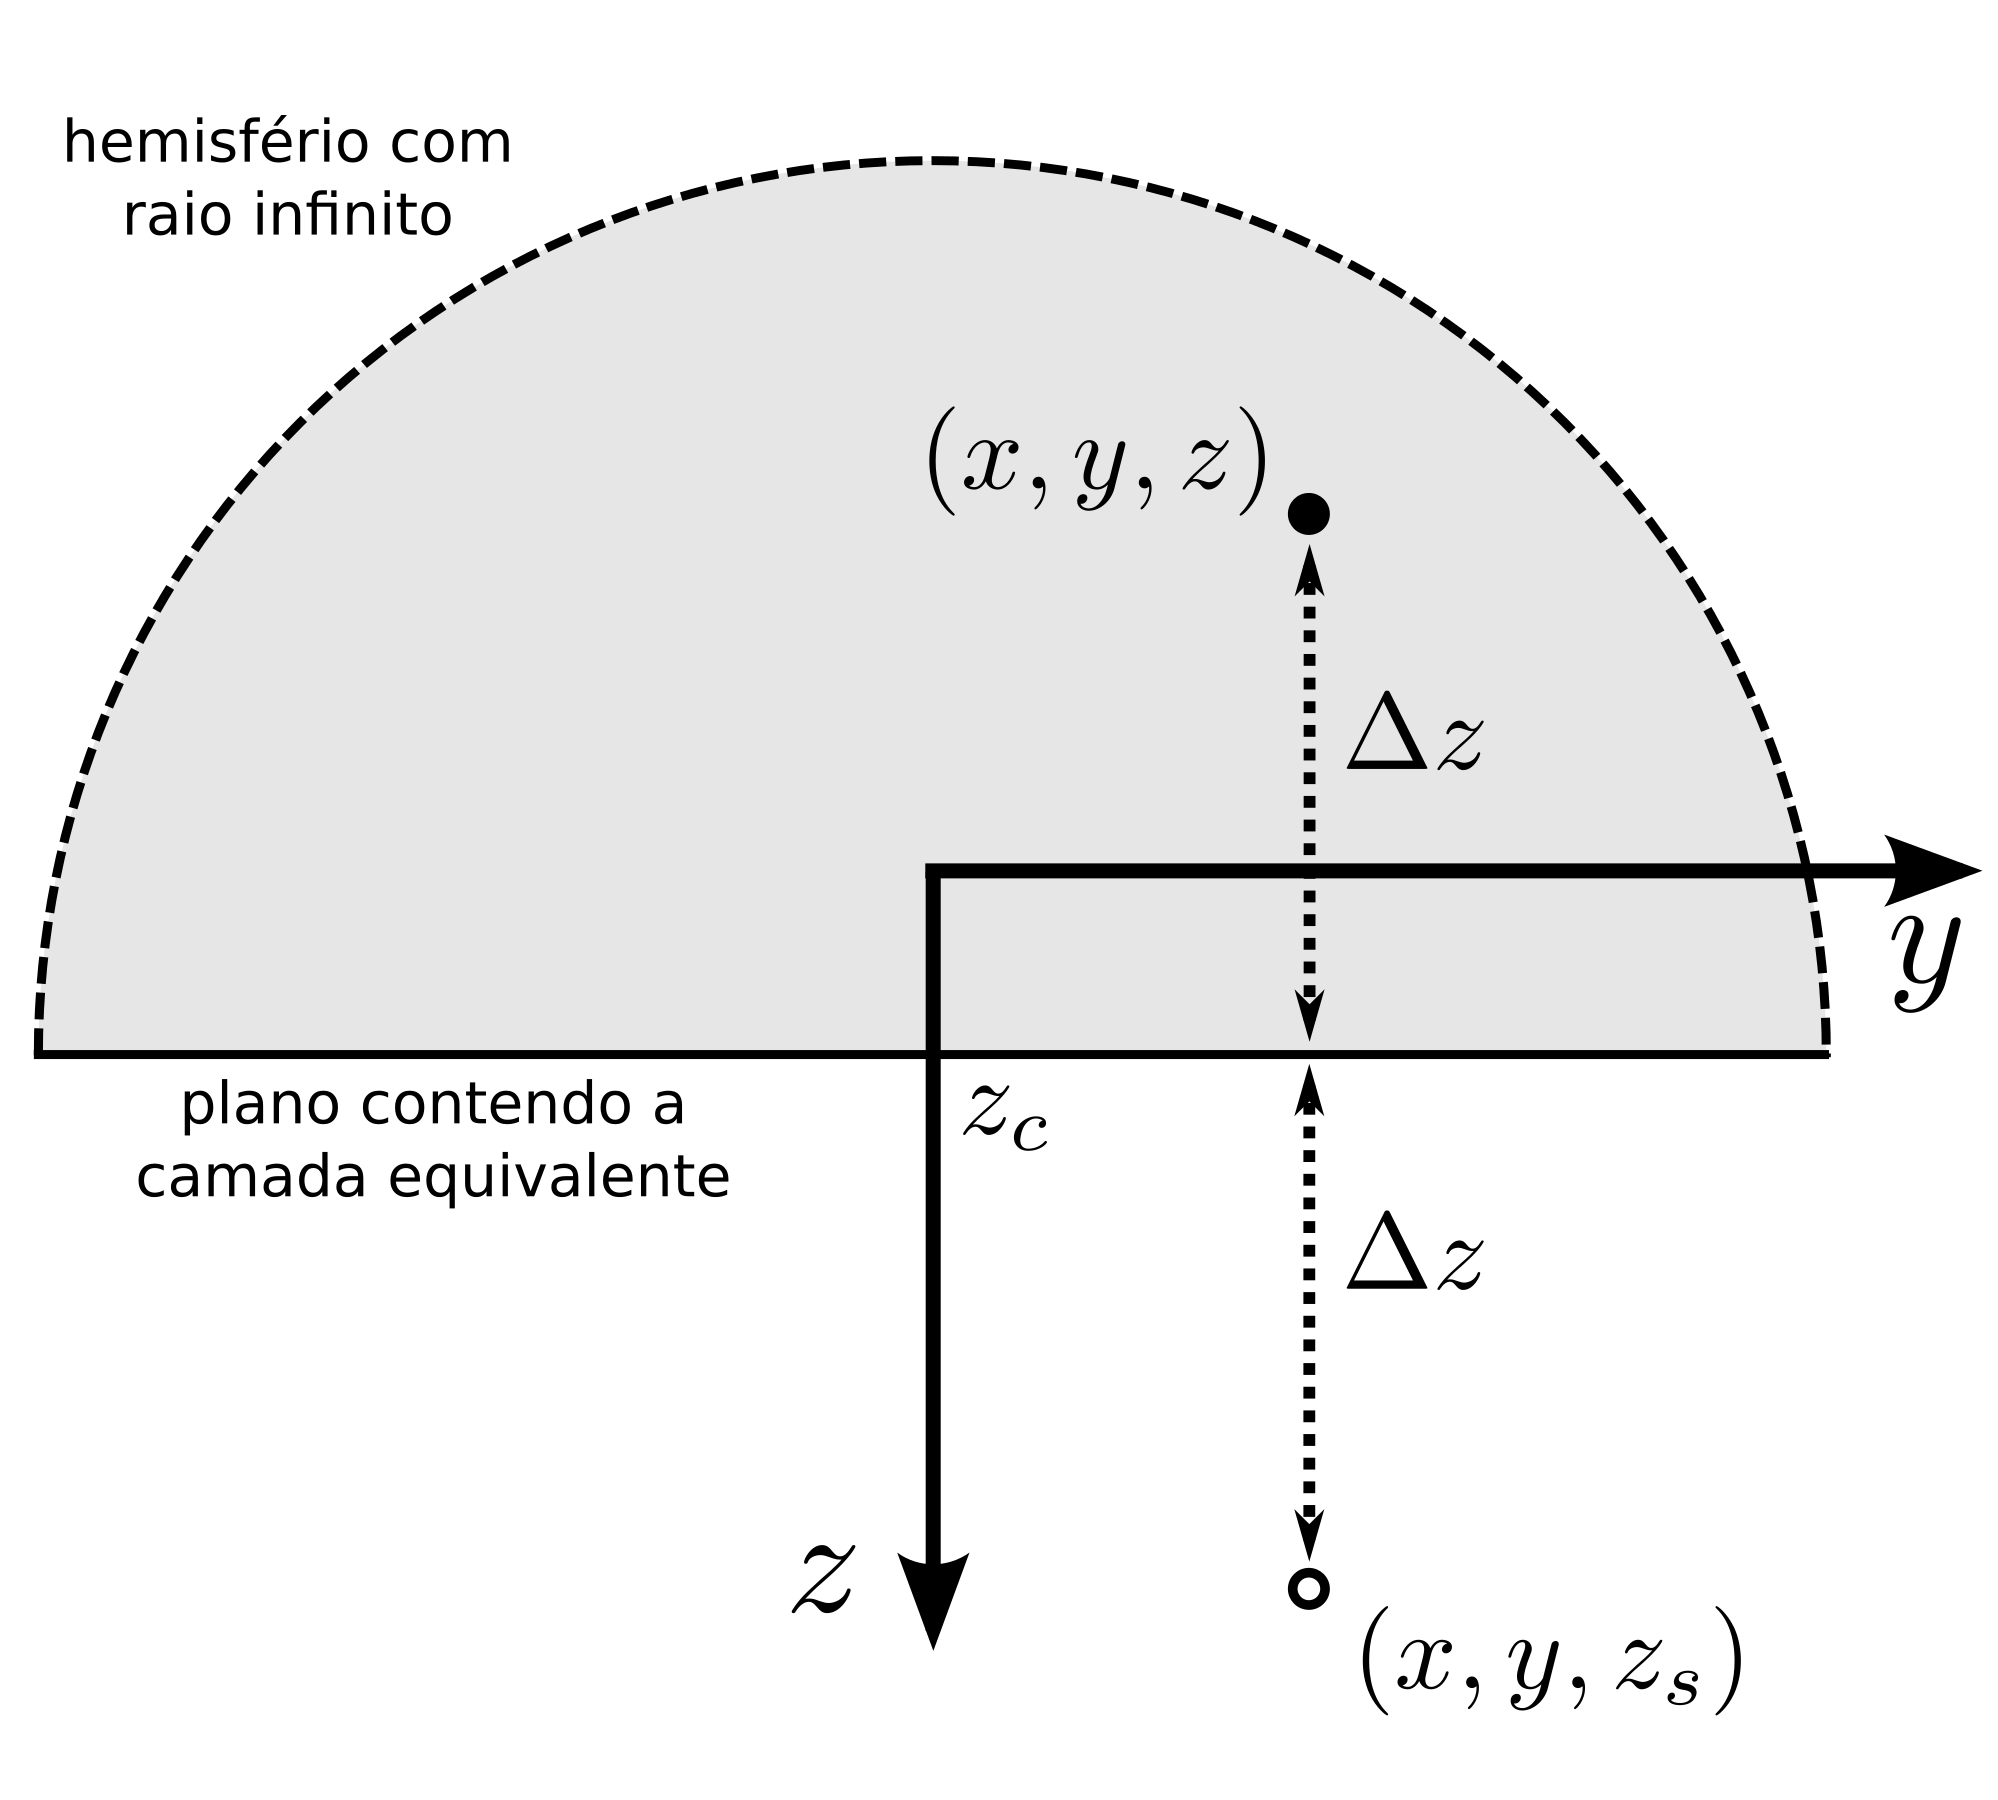
\includegraphics[width=0.75\textwidth]{Fig/eqlayer/surface_Green.png}
	\caption{ Representação 2D da superfícia utilizada para aplicar as identidades de Green. A superfície é formada por uma semi-esfera (linha traçejada) com raio infinito e o plano $z = z_{c}$ contendo a camada equivalente. Os pontos $(x, y, z)$ (ponto fechado) e $(x, y, z_{s})$ (ponto aberto) são posicionados simetricamente com respeito ao plano $z = z_{c}$ e definidos como $z = z_{c} - \Delta z$ e $z = z_{c} + \Delta z$, respectivamente.}
	\label{fig:surface_Green}
\end{figure}